
Our current model with three different weights value can only represent linear separation of the data.
With $W$ representing the slope of the slope of this line in the plan formed by the two variable $x$ and $y$ and the
bias $b$ representing the shift regarding to the origin.

\begin{figure}[h!]
    \begin{center}
        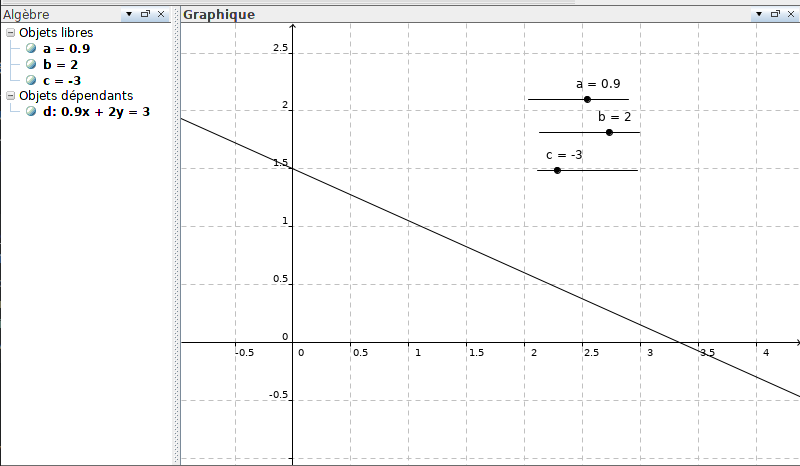
\includegraphics[width=.6\linewidth]{../2_logic_XOR/xor_graph.png}
        \caption{Representation of the the frontier depending on the three weights}
    \end{center}
\end{figure}

But to get an XOR we need to satisfy the following conditions:

\begin{align*}
    f(0,0) &< 0
    f(0,1) &\geq 0
    f(1,0) &\geq 0
    f(1,1) &< 0
\end{align*}

Which is strictly impossible with only one linear boundary.

As a side not it's important to note that:

\[
    XOR(x, y) = \left( \overline{x} \cdot y \right) + ( x \cdot \overline{y} )
\]

So it's possible to have XOR with linear classifier as we already showed how to get $AND$ and $OR$ operations
in subsection \ref{q2.1}.
The $NOT$ operation being just a simple one input classifier with one weight of negative value and no bias.



